\documentclass[10pt,a4paper,twoside]{article}

% Ränder
\addtolength{\topmargin}{-16mm}
\setlength{\oddsidemargin}{25mm}
\setlength{\evensidemargin}{35mm}
\addtolength{\oddsidemargin}{-1in}
\addtolength{\evensidemargin}{-1in}
\setlength{\textwidth}{15cm}
\addtolength{\textheight}{34mm}

%% 	Language and font encodings
\usepackage[T1]{fontenc}									% Standard package for selecting font encodings
\usepackage[utf8]{inputenc}								% Accept different input encodings
\usepackage[english,ngerman]{babel}				% Multilingual support for Plain TEX or LATEX
% \usepackage[ngerman]{babel}						% Multilingual support for Plain TEX or LATEX 

%% 	Useful packages
\usepackage{amsmath} 									% AMS mathematical facilities for LATEX
\usepackage{graphicx}									% Enhanced support for graphics
\usepackage{float}
\usepackage{booktabs} 									% Publication quality tables in LATEX
\usepackage{tabu}										% Flexible LATEX tabulars
\usepackage[colorlinks=true, allcolors=blue]{hyperref}	% Extensive support for hypertext in LATEX
% \usepackage{apacite}									% Citation style following the rules of the APA - comment out if plain style is required
\usepackage[colorinlistoftodos]{todonotes}				% Marking things to do in a LATEX document - [..,prependcaption, textsize=tiny]

%% 	Optional packages
\usepackage{rotating}									% Rotation tools, including rotated full-page floats
\usepackage{enumitem}
\usepackage{xargs}										% Define commands with many optional arguments
% \usepackage{amssymb} 									% To use $\checkmark$
\usepackage{parskip} 								% Entfernt den Einzug bei neuer Zeile und fügt stattdessen einen Abstand ein
\raggedbottom											 % Verhindert zu große Abstände zwischen 


\usepackage{fancyhdr} % Positionierung der Seitenzahlen
\fancyhead[LE,RO,LO,RE]{}
\fancyfoot[CE,CO,RE,LO]{}
\fancyfoot[LE,RO]{\Roman{page}}
\renewcommand{\headrulewidth}{0pt}
\setlength{\headheight}{13.6pt} % behebt headheight Warning

% Korrektes Format für Nummerierung von Abbildungen (figure) und
% Tabellen (table): <Kapitelnummer>.<Abbildungsnummer>
\makeatletter
\@addtoreset{figure}{section}
\renewcommand{\thefigure}{\thesection.\arabic{figure}}
\@addtoreset{table}{section}
\renewcommand{\thetable}{\thesection.\arabic{table}}
\makeatother

% Nicer default font (+ math font) than Computer Modern for most use cases
\usepackage{mathpazo}
\usepackage[mathletters]{ucs} % Extended unicode (utf-8) support

\usepackage{color}
\newcommand{\TODO}[1]{{\color{red}\underline{#1}}}

\usepackage{mdframed}
\newmdenv[
  linecolor = yellow,
  leftmargin = 0pt,
  innerleftmargin = 1em,
  innertopmargin = 0pt,
  innerbottommargin = 0pt,
  innerrightmargin = 0pt,
  rightmargin = 0pt,
  linewidth = 3pt,
  topline = false,
  rightline = false,
  bottomline = false
  ]{leftbar}
% Document parameters
\title{Analysis 1}
\author{}

\begin{document}
\pagestyle{fancy}
\pagenumbering{roman} % Römische Seitenzahlen
\setcounter{page}{1}

\maketitle

\textbf{Informationen zu den Klausuraufgaben:} Die Aufgaben werden sich auf eine Teilmenge der in der Vorlesung behandelten Themen beziehen. Über den folgenden Link gelangen Sie zu einer Seite mit einer 
\href{http://www.math.lmu.de/~philip/teaching/2017_calc1_forInfAndStatStudents/summary.html}{Themenübersicht der bisherigen Vorlesungen}. 
Zur Bearbeitung der Aufgaben wird es dabei notwendig sein, in der Vorlesung erworbenes Verständnis zu demonstrieren sowie in der Vorlesung und in den zugehörigen Übungen erlernte Methoden anzuwenden. Es kann also Aufgaben geben, in denen Sie zeigen sollen, dass Sie den Inhalt wichtiger Definitionen und Sätze aus der Vorlesung verstanden haben. Auch kann es kann Aufgaben geben, bei denen mit den erlernten Methoden etwas zu berechnen oder zu beweisen ist. Die Definitionen und Sätze (ohne Beweise und natürlich ohne Nummern aus dem Skript) der folgenden Liste sollten Sie auswendig wissen und anwenden können (zu den Definitionen sollten Sie Beispiele und Gegenbeispiele angeben können und entscheiden können, ob gegebene Objekte die Definition erfüllen oder nicht). 

% Inhaltsverzeichnis erzeugen
\tableofcontents
\cleardoublepage

% Arabische Seitenzahlen
\pagenumbering{arabic}
\setcounter{page}{1}
% Geändertes Format für Seitenränder, arabische Seitenzahlen
% \fancyhead[LE,RO]{\rightmark}
\fancyhead[LO,RE]{\leftmark}
\fancyfoot[LE,RO]{\thepage}

\section{Logik und Mengenlehre (4-21)}
Definition von logischer Negation, Konjunktion, Disjunktion, Implikation, Äquivalenz. Bestimmung von Wahrheitswerten von Aussageformen. Definition von Gleichheit von Mengen, Teilmenge (Inklusion), Obermenge, Durchschnitt, Vereinigung, Differenz von Mengen, Komplement, Disjunktheit und disjunkte Vereinigung, Potenzmenge. 
\subsection{Definition von logischer Negation, Konjunktion, Disjunktion, Implikation, Äquivalenz. (5f)}
\begin{equation}
\begin{split}
\text{Negation} \qquad & \neg A \\
\text{Konjunktion (and)}  \qquad & A \wedge B \\
\text{Disjunktion (or)}  \qquad & A \vee B \\
\text{Implikation}  \qquad & (A \Rightarrow B) \Leftrightarrow (\neg A \vee B) \Leftrightarrow (\neg B \Rightarrow \neg A) \\
\text{Äquivalenz}  \qquad & (A \Leftrightarrow B) \Leftrightarrow ((A \Rightarrow B) \wedge (B \Rightarrow A))
\end{split}
\end{equation}

\subsection{Bestimmung von Wahrheitswerten von Aussageformen.}

\subsection{Definition von Gleichheit von Mengen, Teilmenge (Inklusion), Obermenge, Durchschnitt, Vereinigung, Differenz von Mengen, Komplement, Disjunktheit und disjunkte Vereinigung, Potenzmenge. (12ff)}
\subsubsection{Gleichheit von Mengen}
$M = N$ wenn alle Elemente von $N$ in $M$ vorkommen. $\Rightarrow$ Wir können nur Aussagen über Mengen treffen wenn wir alle ihre Elemente kennen. $\forall x \in M: x \in N \wedge \forall y \in N: y \in M$
\subsubsection{Teilmenge (Inklusion)}
$M \subseteq N$, wenn alle Elemente aus $M$ in $N$ vorkommen. $\forall x \in M: x \in N$ \\
$M \subset N$, wenn Elemente in $N$ vorhanden sind, die in $M$ nicht vorkommen spricht man von einer echten Teilmenge. $\exists x \in N: x \notin M$

\subsubsection{Obermenge}
Ist $M \subseteq N$, dann ist $N$ die Obermenge von $M$.

Ist $M$ Obermenge von $N$ und umgekehrt, so sind die Mengen äquivalent, $M = N$

\subsubsection{Durschnitt}
$M,N : x \in M \wedge x \in N$
Der Durchschnitt zweier Mengen $M \cap N$ ist die Menge an Elementen, die in beiden Mengen $M$, $N$ vorkommen.

\subsubsection{Vereinigung}
$M,N: x \in M \vee x \in N$
Die Vereinigung zweier Mengen $M \cup N$ ist die Menge an Elementen, die in entweder $M$ oder $N$ vorkommen.

\subsubsection{Differenz von Mengen}
Die Differenz zweier Mengen $M\setminus N$ ist die Menge an Elementen, die in $M$ vorkommen, aber nicht in $N$.
$M,N : x \in M \wedge x \notin N$

\subsubsection{Komplement}
Ist Menge $N$ eine Teilmenge der Menge $M$ ($M \subseteq N$, $M$ ist Universum von $N$), dann wird $M \setminus N$ auch das Komplement $N$ zu $M$ genannt. $N^c := M \setminus N$

\subsubsection{Disjunktheit und disjunkte Vereinigung}
Ist der Durchschnitt zweier Mengen $M \cap N$ die leere Menge, so sind diese Mengen disjunkt. Die Vereinigung zweier disjunkter Mengen lautet dann eine disjunkte Vereinigung und wird $M \dot{\cup} N$ geschrieben.

\subsubsection{Potenzmenge}
Die Potenzmenge einer Menge ist die Menge aller Teilmengen:\\
$M = \{0,1,2\}$, $\mathcal{P}(M)= \{\emptyset, \{0\}, \{1\}, \{2\}, \{0,1\}, \{0,2\}, \{1,2\}, \{0,1,2\}\}$

\section{Funktionen und Relationen (21-33)}
  
Definition der Funktion (insbesondere: Definitionsbereich, Wertebereich, Zuordnungsvorschrift, Graph). Definition von Bild und Urbild einer Menge zu einer gegebenen Funktion. Definition von Injektivität, Surjektivität, Bijektivität, Monotonie (wachsend, streng wachsend, fallend, streng fallend). Definition der Komposition von Abbildungen. Definition der Invertierbarkeit und der inversen Abbildung. Satz: Funktion ist invertierbar genau dann, wenn sie bijektiv ist. Satz: Strenge Monotonie impliziert Injektivität. Definition von oberer Schranke, unterer Schranke, Supremum, Infimum, Beschränktheit von Mengen. Definition der Familie. Definition der Folge. 
Induktion, Rekursion, Kardinalität: 
Beweisprinzip der vollständigen Induktion. Rekursive Definition. Summationssymbol. Produktsymbol. Formel für (endliche) geometrische Summen. Definition von endlich, unendlich, abzählbar. 
\section{Induktion, Rekursion, Kardinalität (33ff)}
Beweisprinzip der vollständigen Induktion. Rekursive Definition. Summationssymbol. Produktsymbol. Formel für (endliche) geometrische Summen. Definition von endlich, unendlich, abzählbar. 

\subsection{Beweisprinzip der vollständigen Induktion (34)}
Induktionsverankerung ($n=1$): Für $n=1$ ergibt sich die Aussage \textbf{TBD} welche wahr ist. Für den
Induktionsschritt sei $n\in\mathbb{N}$. Unter Annahme der Induktionsvoraussetzung \textbf{TBD (1)}, erhält man
\textbf{TBD} was zeigt, dass die Aussage auch für $n+1$ gilt und somit den Induktionsbeweis abschließt.

\begin{itemize}
\item \textbf{IA} $n=1$
\item \textbf{IV} 
\item \textbf{IS} $n \rightarrow n+1$
\end{itemize}

\subsection{Rekursive Definition (36)}
z.B. Fibonacci-Folge
\begin{equation}
\begin{split}
(a_n)_{n \in \mathbb{N}} &= a_{n-1} + a_{n-2} \\ 
a_0 &= 0 \\
a_1 &= 1
\end{split}
\end{equation}

\subsection{Summationssymbol (38)}
\begin{equation}
\begin{split}
\sum\nolimits_{i=1}^1 a_i &:= a_i \\
\sum\nolimits_{i=1}^{n+1} a_i &:=  a_i + \sum\nolimits_{i=1}^{n} \text{für } n \geq 1
\end{split}
\end{equation}

\subsection{Produktsymbol (39)}
\begin{equation}
\begin{split}
\prod\nolimits_{i=1}^1 a_i &:= a_i \\
\prod\nolimits_{i=1}^{n+1} a_i &:= a_i * \prod\nolimits_{i=1}^{n} \text{für } n \geq 1
\end{split}
\end{equation}


\subsection{Formel für (endliche) geometrische Summen (40)}
\begin{figure}[H]
	\centering
  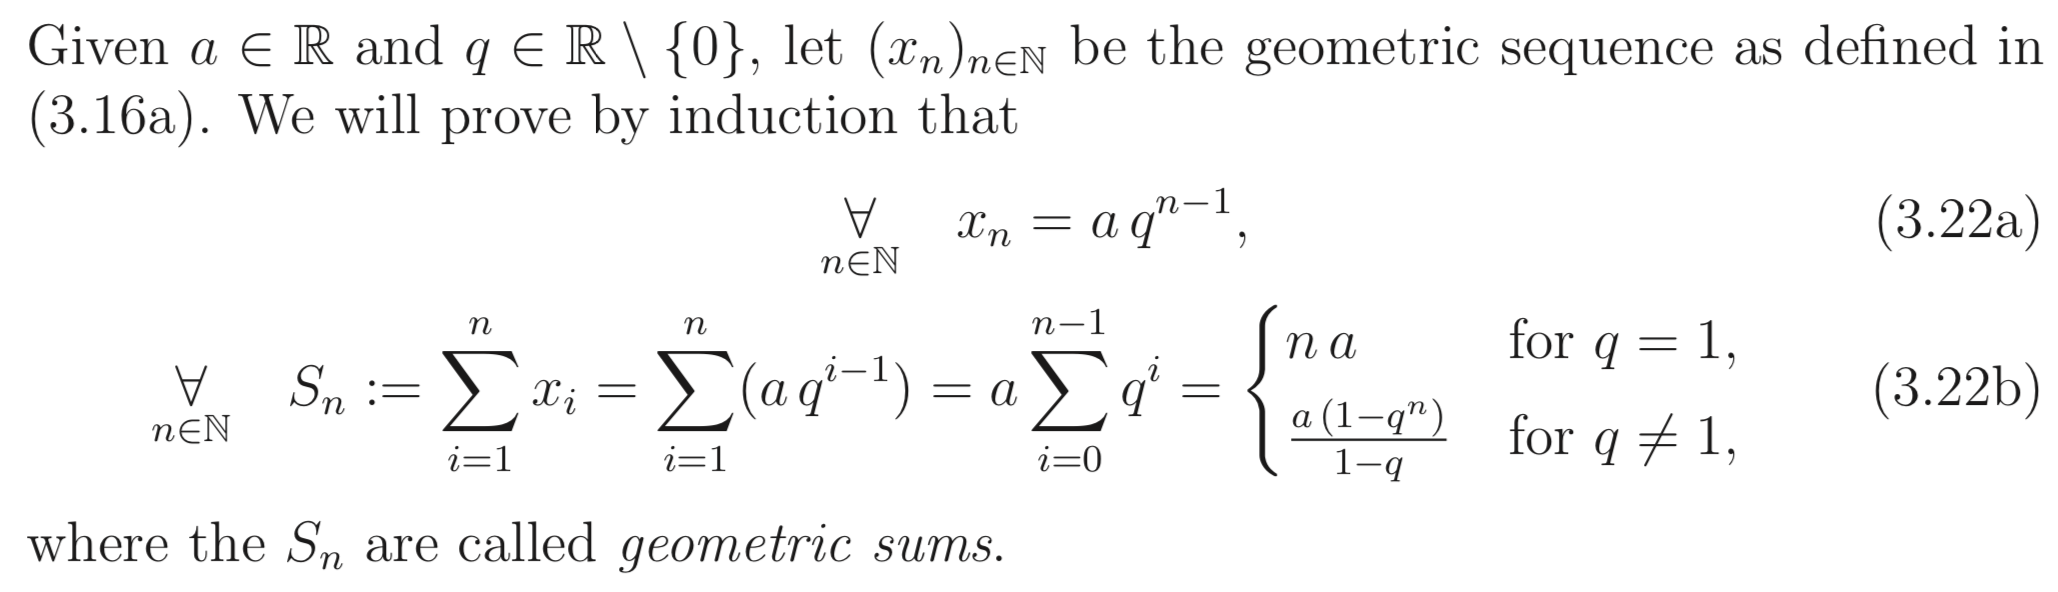
\includegraphics[width=0.7\textwidth]{media/40-example-3-11b.png}
	\caption{40 example 3.11b}
	\label{40_example_3.11b}
\end{figure}

\subsection{Definition von endlich, unendlich, abzählbar (40f)} 
Die Menge $A$ lautet
\begin{itemize}
\item endlich $\Leftrightarrow$ $\exists n \in \mathbb{N_0}$ sodass $\#A = n$ ($\#A :=$ Kardinalität, Anzahl Elemente in $A$)
\item unendlich $\Leftrightarrow$ $A$ ist nicht endlich. ($\#A = \infty$)
\item abzählbar $\Leftrightarrow$ $A$ ist endlich oder $\#A = \#\mathbb{N}$
\end{itemize}

\section{Reelle und komplexe Zahlen}
 
Es wird erwartet, dass Sie die schon aus der Schule bekannten in den natürlichen, rationalen und reellen Zahlen gütigen Rechengesetze beherrschen: Dazu gehören die in Theorem 4.6 und Theorem 4.7 im Skript aufgelisteten Gesetze, insbesondere die Bruchrechnung, sowie die binomischen Formeln und die Potenzgesetze. Definition von Intervallen (alle Typen aus (4.11) sollten Sie kennen). Definition der komplexen Zahlen als Paare reeller Zahlen, Definition der komplexen Addition und Multiplikation. Definition von Realteil und Imaginärteil komplexer Zahlen. Definition von und Rechenregeln für komplexe/r Konjugation. Definition der Betragsfunktion reeller und komplexer Zahlen. Rechenregeln der Betragsfunktion, speziell Dreiecksungleichung und umgekehrte Dreiecksungleichung. Veranschaulichung der komplexen Zahlen und ihrer Arithmetik (speziell von Konjugation, Addition, Multiplikation und Betrag) in der komplexen Ebene. Regeln für endliche Summen und Produkte. 

\section{Funktionsarithmetik und Polynome (63-67)}
 
Die punktweise definierte Arithmetik reell- und komplexwertiger Funktionen. Monome und Polynome. Grad von Polynomen. 

\subsection{Punktweise definierte Arithmetik reell- und komplexwertiger Funktionen (63)}
\TODO{Notation 6.1, 6.2}

\subsection{Monome und Polynome}
\TODO{Defintion 6.3}

\subsection{Grad von Polynomen}
\TODO{Theorem 6.6}

\section{Konvergenz reeller und komplexer Folgen (67-105)}
 
Definition und Veranschaulichung der Epsilon-Umgebung sowie der Umgebung einer reellen Zahl sowie einer komplexen Zahl. Definition der Beschränktheit reeller und komplexer Folgen. Definition von Konvergenz und Grenzwert/Limes reeller und komplexer Folgen. Definition von Divergenz reeller und komplexer Folgen. Satz: Konvergente Folgen sind beschränkt. Nullfolgen sind solche, die gegen Null konvergieren. Satz: Eine durch eine Nullfolge beschränkte Folge ist selbst eine Nullfolge. Satz: Das Produkt aus einer Nullfolge und einer beschränkten Folge ist eine Nullfolge. Die Grenzwertsätze aus Th. 7.13 wissen und zur Bestimmung von Grenzwerten anwenden können. Einschachtelungssatz. Definition der bestimmten Divergenz gegen plus oder minus Unendlich. Eine monoton steigende Folge konvergiert oder divergiert bestimmt gegen plus Unendlich; eine monoton fallende Folge konvergiert oder divergiert bestimmt gegen minus Unendlich. Definition von Teilfolge und Umordnung einer Folge. Satz: Jede Teilfolge und jede Umordnung einer konvergenten Folge ist konvergent mit dem selben Limes. 


\subsection{Definition und Veranschaulichung der Epsilon-Umgebung sowie der Umgebung einer reellen Zahl sowie einer komplexen Zahl}
Die Menge $A \subset \mathbb{K}$ ist eine Umgebung von $x \Leftrightarrow$ 
$\exists \epsilon > 0 : B_{\epsilon}(x) = \{x' \in \mathbb{K} : |x'-x| < \epsilon\}$
$B_{\epsilon} \subset A$

“Die Menge aller $x'$ die weniger als $\epsilon$ von $x$ entfernt sind.”

\TODO{TODO}

\subsection{Definition der Beschränktheit reeller und komplexer Folgen (69)}
The sequence $(z _ { n }) _ { n \in \mathbb { N } }$  in $\mathbb{K}$ is called bounded if, and only if, the set
$\left\{ | z _ { n } | : n \in \mathbb { N } \right\}$ is bounded in the sense of Def. 2.26(a).

\subsection{Definition von Konvergenz und Grenzwert/Limes reeller und komplexer Folgen}

Die reelle Zahl $z$ heißt \textit{Grenzwert} oder \textit{Limes} der Zahlenfolge $\left\langle z _ { n } \right\rangle$, wenn es zu jedem $\epsilon > 0$ eine positive Zahl $N$
 gibt, so dass für alle $n > N$ stets $| z _ { n } - z | < \epsilon$ ist.
 
 Eine Folge $\left\langle z _ { n } \right\rangle$ heißt \textit{konvergent}, wenn sie einen \textit{Grenzwert} $z$ besitzt $\Leftrightarrow \lim\limits_ { n \rightarrow \infty } z _ { n } = z$.
 
\textbf{Kurz gefasst:} Sei $(z_n)_{n \in \mathbb{N}}$ Folge.\\
$z_n$ ist konvergent $\Leftrightarrow$ 
$\lim\limits_{n \rightarrow \infty}{z_n} = z \Leftrightarrow$ 
$\underset{\epsilon \in \mathbb{R^+}}{\forall} \ \underset{N \in \mathbb{N}}{\exists} \ \underset{n > N}{\forall} \  |z_n - z| < \epsilon$
\newline
\begin{leftbar}
 Beispiel:
\begin{itemize}
 \item Es sei $z_n = \frac{1}{n}$ unsere Folge.
 \item Berechne Grenzwert: $\lim\limits_{n \rightarrow \infty}{z_n} = 0$
 \item Schreibe: Sei $e \in \mathbb{R^+}$, wähle $N = ?$, sei $n > N$
 \item Setze $a_n$ und $a$ ein: $|z_n - 0| = |\frac{1}{n} -0| = {|\frac{1}{n}| < \frac{1}{N}} = \epsilon$
 \item $\Rightarrow N = \frac{1}{\epsilon}$
 \end{itemize} 
 \end{leftbar}
 
 \TODO{68 Komplexe Zahl Konvergenz}
 
 \TODO{69-Def.7.7 (Neighborhood)}


\subsection{Definition von Divergenz reeller und komplexer Folgen}
\TODO{TODO}

\subsection{Satz: Konvergente Folgen sind beschränkt (69)}
Let $(z _ { n }) _ { n \in \mathbb { N } }$ be a sequence in $\mathbb{K}$. If  $(z _ { n }) _ { n \in \mathbb { N } }$  is convergent, then it is bounded.

\subsection{Nullfolgen sind solche, die gegen Null konvergieren (70)}
Let $(z _ { n }) _ { n \in \mathbb { N } }$ be a sequence in $\mathbb{C}$ with $\lim _ { n \rightarrow \infty } z _ { n } = 0$.

\subsubsection{Satz: Eine durch eine Nullfolge beschränkte Folge ist selbst eine Nullfolge (70)}
If $(b _ { n }) _ { n \in \mathbb { N } }$ is a sequences in $\mathbb{C}$ such that there exists $C \in \mathbb { R } ^ { + }$ with $| b _ { n } | \leq C | z _ { n } |$ for
almost all $n$, then $\lim _ { n \rightarrow \infty } b _ { n } = 0$.

\subsubsection{Satz: Das Produkt aus einer Nullfolge und einer beschränkten Folge ist eine Nullfolge (70)}
If $(c _ { n }) _ { n \in \mathbb { N } }$ is a bounded sequence in $\mathbb{C}$, then $\lim _ { n \rightarrow \infty } (c_n z_n) = 0$.

\subsection{Die Grenzwertsätze aus Th. 7.13 wissen und zur Bestimmung von Grenzwerten anwenden können (70f)}
\textit{Siehe Skript} \newline
\begin{leftbar}
Seite 70-71
\end{leftbar}

\subsection{Einschachtelungssatz (Sandwich Theorem) (72)}
Let $(x _ { n }) _ { n \in \mathbb { N } }$, $(y _ { n }) _ { n \in \mathbb { N } }$, and $(a _ { n }) _ { n \in \mathbb { N } }$ be sequences in $\mathbb{R}$. If $x _ { n } \leq a _ { n } \leq y _ { n }$ holds for almost all $n \in \mathbb { N }$, then
\begin{equation}
\lim _ { n \rightarrow \infty } x _ { n } = \lim _ { n \rightarrow \infty } y _ { n } = x \in \mathbb { R } \quad \Rightarrow \quad \lim _ { n \rightarrow \infty } a _ { n } = x
\end{equation} \newline
\begin{leftbar}
Sei $(x_n)_{x \in \mathbb{N}}, (y_n)_{y \in \mathbb{N}}$ Folgen. Wenn $x_n \leq a_n \leq y_n$ für fast alle $n$.

Dann $\lim\limits_{n \rightarrow \infty}{x_n} = \lim\limits_{n \rightarrow \infty}{y_n} = x \in \mathbb{R} \Rightarrow$
$\lim\limits_{n \rightarrow \infty}{a_n} = x$
\end{leftbar}

\subsection{Definition der bestimmten Divergenz gegen plus oder minus Unendlich (72)}
Let $(x _ { n }) _ { n \in \mathbb { N } }$ be a sequence in $\mathbb{R}$. The sequence is said to diverge to
$\infty$ (resp. to $-\infty$), denoted $\lim _ { n \rightarrow \infty } x _ { n } = \infty$ (resp. $\lim _ { n \rightarrow \infty } x _ { n } = -\infty$) if, and only if, for
each $K \in \mathbb { R }$, almost all $x_n$ are bigger (resp. smaller) than $K$. Thus,
\begin{align}
\lim _ { n \rightarrow \infty } x _ { n } = \infty \quad & \Leftrightarrow \underset{K \in \mathbb{R}}{\forall} \ \underset{N \in \mathbb{N}}{\exists} \ \underset{n > N}{\forall}  \ x _ { n } > K \\
\lim _ { n \rightarrow \infty } x _ { n } = -\infty \quad & \Leftrightarrow \underset{K \in \mathbb{R}}{\forall} \ \underset{N \in \mathbb{N}}{\exists} \ \underset{n > N}{\forall}  \ x _ { n } < K
\end{align}

\subsection{Eine monoton steigende Folge konvergiert oder divergiert bestimmt gegen plus Unendlich; eine monoton fallende Folge konvergiert oder divergiert bestimmt gegen minus Unendlich (73)}
Suppose $S := (x_n)_{n \in \mathbb{N}}$ is a monotone sequence in $\mathbb{R}$ (increasing or decreasing). Defining $A := \{x_n : n \in \mathbb{N}\}$, the following holds:
\begin{equation}
\lim\limits_{n\rightarrow \infty}x_n =
\begin{cases}
\text{sup}A & \text{if $S$ is increasing and bounded,} \\
\infty & \text{if $S$ is increasing and not bounded,} \\
\text{inf}A & \text{if $S$ is decreasing and bounded,} \\
-\infty & \text{if $S$ is decreasing and not bounded.}
\end{cases}
\end{equation}

\subsection{Definition von Teilfolge und Umordnung einer Folge (73)}
Let $A$ be an arbitrary nonempty set. Consider a sequence $\sigma : \mathbb { N } \rightarrow A$. Given a function $\phi : \mathbb { N } \rightarrow \mathbb { N }$ (that means $( \phi ( n ) ) _ { n \in \mathbb { N } }$ constitutes a sequence of
indices), the new sequence $( \sigma \circ \phi ) : \mathbb { N } \rightarrow A$ is called a subsequence of $\sigma$ if, and
only if, $\phi$ is strictly increasing (i.e. $1\leq \phi ( 1) < \phi ( 2) < \dots$ ). Moreover, $ \sigma \circ \phi$ is
called a reordering of $\sigma$ if, and only if, $\phi$ is bijective. One can write $\sigma$ in the form
$(z_{ n }) _ { n \in \mathbb { N } }$ by setting $z _ { n } : = \sigma ( n )$, and one can write $ \sigma \circ \phi$  in the form $\left( w _ { n } \right) n \in \mathbb { N }$ by setting
$w _ { n } : = ( \sigma \circ \phi ) ( n ) = z _ { \phi ( n ) }$. Especially for a subsequence of $(z_{ n }) _ { n \in \mathbb { N } }$, it is also common
to write $\left( z _ { n _ { k } } \right) _ { k \in \mathbb { N } }$. This notation corresponds to the one above if one lets $n _ { k } : = \phi ( k )$.
Analogous definitions work if the index set $\mathbb{N}$ of $\sigma$ is replaced by a general countable nonempty index set $I$. \newline
\begin{leftbar}
\textbf{Example:} Consider the sequence $(1, 2, 3, \dots )$. Then $(2, 4, 6, \dots )$ constitutes a subsequence and $(2, 1, 4, 3, 6, 5, \dots )$ constitutes a reordering. Using the notation of Def. 7.21, the original sequence is given by $\sigma : \mathbb { N } \rightarrow \mathbb { N }$, $\sigma ( n ) : = n$; the subsequence
is selected via $\phi _ { 1} : \mathbb { N } \rightarrow \mathbb { N }$, $\phi _ { 1} ( n ) : = 2n$; and the reordering is accomplished via
\begin{equation}
\phi _ { 2} : \mathbb { N } \rightarrow \mathbb { N } ,\phi _ { 2} ( n ) : =
\begin{cases}
n + 1 & \text{if $n$ is odd,} \\
n - 1 & \text{if $n$ is even.}
\end{cases}
\end{equation}
\end{leftbar}

\subsection{Satz: Jede Teilfolge und jede Umordnung einer konvergenten Folge ist konvergent mit dem selben Limes (73)}
Let $\left( z _ { n } \right) n \in \mathbb { N }$ be a sequence in $\mathbb{C}$. If $\lim _ { n \rightarrow \infty } z _ { n } = z$, then every
subsequence and every reordering of $\left( z _ { n } \right) n \in \mathbb { N }$ is also convergent with limit $z$.
\section{Stetigkeit plus Zubehör}
 
Definition der Stetigkeit von Funktionen, die auf Teilmengen der komplexen (oder reellen) Zahlen definiert sind und in die reellen oder komplexen Zahlen abbilden. Folgenkriterium für Stetigkeit. Sie sollten einfache Stetigkeitsbeweise sowohl mit dem Epsilon-Delta-Kriterium als auch mit dem Folgenkriterium durchföhren können. Satz: Sind zwei Funktionen stetig, so auch Vielfache, die Summe, das Produkt, der Quotient, falls der Nenner nicht Null ist, der Betrag der Funktion sowie der Realteil und der Imaginärteil der Funktion. Satz: Eine komplexwertige Funktion ist genau dann stetig, wenn ihr Realteil und ihr Imaginärteil beide stetig sind. Satz: Betragsfunktion, Polynome und rationale Funktionen sind stetig, sofern der Nenner nicht Null ist. Satz: Die Komposition stetiger Funktionen ist stetig. Definition von beschränkten, abgeschlossenen und kompakten Teilmengen der komplexen Zahlen. Beschränkte Intervalle sind beschränkt, abgeschlossene Intervalle sind abgeschlossen. Offene und halboffene Intervalle sind nicht abgeschlossen. Nur Intervalle der Form [a,b] sind kompakt. Epsilon-Umgebungen sind beschränkt, aber nicht abgeschlossen. Endliche Vereinigungen und beliebige Durchschnitte erhalten Beschränktheit, Abgeschlossenheit und Kompaktheit. Endliche Mengen sind kompakt. Urbilder von abgeschlossenen Mengen unter stetigen Abbildungen sind abgeschlossen. Abgeschlossene Kreisscheiben und Kreise sind kompakt. Halbräume in den komplexen Zahlen sind abgeschlossen. Satz: Stetige Bilder kompakter Mengen sind kompakt. Definition globaler und lokaler Extrema ((strenge) Minima und Maxima). Satz: Stetige Abbildungen auf kompakten Mengen nehmen ihr (globales) Maximum und Minimum an. Nullstellensatz von Bolzano, Zwischenwertsatz, stetige Funktionen bilden Intervalle auf Intervalle ab. Definition der n.ten Wurzel einer nichtnegativen Zahl; die zugehörige Funktion ist stetig und streng monoton steigend. Nicht rationale Zahlen heißen irrational; die Menge der rationalen Zahlen ist abzählbar; die Menge der irrationalen Zahlen ist nicht abzählbar. Definition der Dichtheit einer Menge in den reellen Zahlen. Satz: Die rationalen Zahlen sind dicht in den reellen Zahlen; die irrationalen Zahlen sind ebenfalls dicht. Satz: Jede reelle Zahl ist der Grenzwert einer streng steigenden Folge rationaler Zahlen und einer streng fallenden Folge rationaler Zahlen. Definition von Potenzen mit nichtnegativer Basis und reellen Exponenten; es gelten die üblichen Potenzgesetze. Definition von allgemeinen Potenzfunktionen und Exponentialfunktionen. Satz: Potenzfunktionen sind auf ihrem jeweiligen Definitionsbereich stetig, sowie streng steigend für positiven und streng fallend für negativen Exponenten. Satz: Exponentialfunktionen sind stetig sowie streng steigend für Basis a>1 und streng fallend für Basis 0 < a < 1. Definition des Logarithmus, speziell des natürlichen Logarithmus, Logarithmengesetze gemäß Th. 7.75. 
\section{Unendliche Reihen}
 
Definition von unendlichen Reihen sowie von Summanden, Partialsummen und Resten von solchen Reihen. Definition von Konvergenz und Divergenz von Reihen. Geometrische Reihen mit Formel für den Grenzwert. Linearität, komplexe Konjugation und Monotonie bei der Reihenkonvergenz. Satz: Bei konvergenten Reihen konvergieren die Summanden gegen Null. Satz: Die Summe einer Reihe mit nichtnegativen Summanden ist das Supremum der Partialsummen, wenn diese beschränkt sind und andernfalls unendlich. Satz: Eine beliebige Reihe ist konvergent, wenn sich die Beträge ihrer Summanden nach oben durch die Summanden einer konvergenten Reihe abschätzen lassen; eine Reihe mit nichtnegativen Summanden ist divergent, wenn sich ihre Summanden nach unten durch die Summanden einer divergenten Reihe mit ebenfalls nichtnegativen Summanden abschätzen lassen. Definition der absoluten Konvergenz von Reihen. Satz: Absolut konvergente Reihen sind konvergent, und es gilt die Dreiecksungleichung für unendliche Reihen. Wurzelkriterium und Quotientenkriterium jeweils für absolute Konvergenz bzw. für Divergenz. Definition der punktweisen und der gleichmäßigen Konvergenz von Funktionenfolgen bestehend aus reell- oder komplexwertigen Funktionen. Satz: Gleichmäßige Konvergenz impliziert punktweise Konvergenz, aber nicht umgekehrt. Satz: Konvergieren stetige Funktionen gleichmäßig, so ist die Grenzfunktion ebenfalls stetig. Definition von Funktionenreihen, speziell Definition von Potenzreihen. Definition der punktweisen und gleichmäßigen Konvergenz von Funktionenreihen (man spricht von Reihenentwicklung bzw. Potenzreihenentwicklung der Grenzfunktion). Konvergiert eine Funktionenreihe stetiger Funktionen gleichmäßig, so ist die Grenzfunktion stetig. Definition des Konvergenzradius und Formeln zur Berechnung des Konvergenzradius von Potenzreihen. Satz: Potenzreihen sind auf auf dem offenen r-Kreis um Null stetig, wenn r der Konvergenzradius ist. Definition der komplexen Exponentialfunktion als Potenzreihe. Satz: Die komplexe Exponentialfunktion ist stetig und stimmt auf den reellen Zahlen mit der früher definierten Exponentialfunktion überein. Definition des Limes einer reell- oder komplexwertigen Funktion. Definition von Potenzen mit positiver Basis und komplexen Exponenten, dazu Potenzgesetze und Stetigkeit der nun allgemeineren Potenz- und Exponentialfunktionen. 


\subsection{Definition von unendlichen Reihen sowie von Summanden, Partialsummen und Resten von solchen Reihen.}
TODO
\subsection{Definition von Konvergenz und Divergenz von Reihen.}

\subsection{Geometrische Reihen mit Formel für den Grenzwert.}

\subsection{Linearität, komplexe Konjugation und Monotonie bei der Reihenkonvergenz.}
TODO
\subsection{Satz: Bei konvergenten Reihen konvergieren die Summanden gegen Null.}

\subsection{Satz: Die Summe einer Reihe mit nichtnegativen Summanden ist das Supremum der Partialsummen, wenn diese beschränkt sind und andernfalls unendlich.}
TODO
\subsection{Satz: Eine beliebige Reihe ist konvergent, wenn sich die Beträge ihrer Summanden nach oben durch die Summanden einer konvergenten Reihe abschätzen lassen; eine Reihe mit nichtnegativen Summanden ist divergent, wenn sich ihre Summanden nach unten durch die Summanden einer divergenten Reihe mit ebenfalls nichtnegativen Summanden abschätzen lassen.}

\subsection{Definition der absoluten Konvergenz von Reihen.}

TODO
\subsection{Satz: Absolut konvergente Reihen sind konvergent, und es gilt die Dreiecksungleichung für unendliche Reihen.}


\subsection{Wurzelkriterium und Quotientenkriterium jeweils für absolute Konvergenz bzw. für Divergenz.}
TODO
\subsection{Definition der punktweisen und der gleichmäßigen Konvergenz von Funktionenfolgen bestehend aus reell- oder komplexwertigen Funktionen.}

\subsection{Satz: Gleichmäßige Konvergenz impliziert punktweise Konvergenz, aber nicht umgekehrt.}
TODO
\subsection{Satz: Konvergieren stetige Funktionen gleichmäßig, so ist die Grenzfunktion ebenfalls stetig.}

\subsection{Definition von Funktionenreihen, speziell Definition von Potenzreihen.}
TODO
\subsection{Definition der punktweisen und gleichmäßigen Konvergenz von Funktionenreihen (man spricht von Reihenentwicklung bzw. Potenzreihenentwicklung der Grenzfunktion).}

\subsection{Konvergiert eine Funktionenreihe stetiger Funktionen gleichmäßig, so ist die Grenzfunktion stetig.}
TODO
\subsection{Definition des Konvergenzradius und Formeln zur Berechnung des Konvergenzradius von Potenzreihen.}

\subsection{Satz: Potenzreihen sind auf auf dem offenen r-Kreis um Null stetig, wenn r der Konvergenzradius ist.}
TODO
\subsection{Definition der komplexen Exponentialfunktion als Potenzreihe.}

\subsection{Satz: Die komplexe Exponentialfunktion ist stetig und stimmt auf den reellen Zahlen mit der früher definierten Exponentialfunktion überein.} 
TODO
\subsection{Definition des Limes einer reell- oder komplexwertigen Funktion.}

\subsection{Definition von Potenzen mit positiver Basis und komplexen Exponenten, dazu Potenzgesetze und Stetigkeit der nun allgemeineren Potenz- und Exponentialfunktionen.}

TODO
\section{Trigonometrische Funktionen (115-126)}
 
Sie brauchen NICHT die Potenzreihendefinition von Sinus und Kosinus auswendig wissen, sondern nur jeweils den schon aus der Schule bekannten groben Verlauf des reellen Sinus und des reellen Kosinus (also im Wesentlichen die Grafen mit Lage der Nullstellen, Maxima, Minima und Monotoniebereichen sowie sin*sin+cos*cos=1 - das beeinhaltet die Eigenschaften aus Th. 8.22 außer den Additionstheoremen und den Grenzwerten). Sie sollten auch wissen, dass sin und cos auf den ganzen komplexen Zahlen definiert und stetig sind. Eulersche Formel (8.46a). Definition von Tangens und Cotangens, ebenfalls mit Nullstellen und Monotonieintervallen. Polarkoordinaten komplexer Zahlen (Betrag,Argument). Darstellung in der komplexen Ebene. Multiplikation komplexer Zahlen in Polarkoordinaten. 

\subsection{reeller Sinus, reeller Cosinus}
\begin{figure}[H]
	\centering
  \includegraphics[width=\linewidth]{../img/{sin-cos}.png}
	\caption{sin-cos}
	\label{sin-cos}
\end{figure}

\begin{table}[H]
%\centering
\begin{tabular}{|l||l|l|}
\hline
Eigenschaften ( $k \in \mathbb { Z }$ )     & $y= sin x$ & $y = cos x$ \\ \hline \hline
Definitionsbereich &     $- \infty < x < \infty$     &    $- \infty < x < \infty$       \\
Wertebereich       &    $ - 1\leq y \leq 1 $    &     $- 1\leq y \leq 1   $   \\ 
Periode (primitive)           &     $ 2\pi $   &    $ 2\pi  $    \\ 
Symmetrie          &     ungerade     &     gerade      \\ 
Nullstellen        &     $x _ { k } = k \cdot \pi$     &     $x _ { k } = \frac { \pi } { 2} + k \cdot \pi$      \\ 
Relative Maxima    &    $x _ { k } = \frac { \pi } { 2} + k \cdot 2\pi$      &      $x _ { k } = k \cdot 2\pi$     \\
Relative Minima    &     $x _ { k } = \frac { 3} { 2} \pi + k \cdot 2\pi$     &    $x _ { k } = \pi + k \cdot 2\pi$       \\ \hline
\end{tabular}
\caption{sin-cos-tab}
\label{sin-cos-tab}
\end{table}

Theorem 8.22
\begin{equation}
sin 0 = 0, \qquad cos 0 = 1
\end{equation}
\begin{equation}
\forall _ { z \in \mathbb { C } } \qquad\sin z = - \sin ( - z ) ,\qquad \cos z = \cos ( - z )
\end{equation}
\begin{equation}
\forall _ { z \in \mathbb { C } }  \qquad( \sin z ) ^ { 2} + ( \cos z ) ^ { 2} = 1
\end{equation}
\begin{equation}
\cos \frac { \pi } { 2} = 0,\quad \sin \frac { \pi } { 2} = 1,\quad \forall _ { x \in [ 0,\frac { \pi } { 2} } ] \cos x > 0
\end{equation}

\subsection{sin und cos sind auf den ganzen komplexen Zahlen definiert und stetig}

\subsection{Eulersche Formel (120)}
\begin{equation}
\underset{ z \in \mathbb { C } }{\forall} e ^ { i z } = \cos z + i \sin z
\end{equation}

\subsection{reeller Tangens, reeller Kotangens}
\begin{figure}[H]
	\centering
  \includegraphics[width=\linewidth]{../img/{tan-cotan}.png}
	\caption{tan-cotan}
	\label{tan-cotan}
\end{figure}

\begin{table}[H]
%\centering
\begin{tabular}{|l|l|l|}
\hline
Eigenschaften    ( $k \in \mathbb { Z }$ )     & $y= tan x$ & $y= cot x$ \\ \hline \hline
Definitionsbereich    &    \parbox[t]{2in}{ $x \in \mathbb { R }$ mit Ausnahme der Stellen \par  $x _ { k } = \frac { \pi } { 2} + k \cdot \pi$   }  &   \parbox[t]{2in}{   $x \in \mathbb { R }$ mit Ausnahme der Stellen  \par  $x _ { k } =  k \cdot \pi$   }    \\ 
Wertebereich          &   $- \infty < y < \infty$       &  $- \infty < y < \infty$          \\ 
Periode (primitive)   &   $\pi$       &      $\pi$     \\ 
Symmetrie             &    ungerade      &  ungerade         \\ 
Nullstellen           &     $x _ { k } = k \cdot \pi$     &      $x _ { k } = \frac { \pi } { 2} + k \cdot \pi$     \\ 
Pole                  &    $x _ { k } = \frac { \pi } { 2} + k \cdot \pi$      &    $x _ { k } = k \cdot \pi$       \\ 
Senkrechte Asymptoten &    $x = \frac { \pi } { 2} + k \cdot \pi$      &      $x = k \cdot \pi$        \\ \hline
\end{tabular}
\caption{tan-cotan-tab}
\label{tan-cotan-tab}
\end{table}

\begin{leftbar}
\noindent\begin{minipage}{.5\linewidth}
\begin{equation}
\tan x = \frac { \sin x } { \cos x } = \frac { 1} { \cot x }
\end{equation}
\end{minipage}
\begin{minipage}{.5\linewidth}
\begin{equation}
\cot x = \frac { \cos x } { \sin x } = \frac { 1} { \tan x }
\end{equation}
\end{minipage}
\end{leftbar}

\subsection{Polarkoordinaten komplexer Zahlen (Betrag, Argument) (123)}
For each complex number $z \in \mathbb { C }$, there exist real numbers $r\geq 0$ and $\varphi \in \mathbb { R }$ such that
\begin{equation}
z = r e ^ { i \varphi }
\end{equation}
$r :=$ Betrag, $\varphi :=$ Argument

\TODO{TODO}

\subsection{Darstellung in der komplexen Ebene (124)}
\TODO{TODO}

\subsection{Multiplikation komplexer Zahlen in Polarkoordinaten (124)}
\TODO{TODO}
\section{Differentialrechnung}
 
Definition der Differenzierbarkeit und Ableitung für reell- und für komplexwertige Funktionen. Satz: Eine komplexwertige Funktion ist genau dann differenzierbar, wenn ihr Realteil und ihr Imaginärteil differenzierbar sind. Satz: Differenzierbarkeit impliziert Stetigkeit. Ableitungsregeln: Ableiten ist linear, Produktregel, Quotientenregel, Kettenregel. Ableitungen von Polynomen, von der reellen Exponentialfunktion, vom natürlichen Logarithmus, vom reellen Sinus und vom reellen Kosinus. Ableitung von Potenzfunktionen mit reellen Exponenten. Definition von Ableitungen höherer Ordnung. Satz: Ist eine Funktion in einem lokalen Extremum differenzierbar, so verschwindet dort die Ableitung, Satz über den Zusammenhang des Vorzeichens der Ableitung mit der Monotonie einer differenzierbaren Funktion. Hinreichende Bedingungen für die Existenz von Maxima und Minima bei differenzierbaren Funktionen. 
\section{Riemannintegral auf kompakten Intervallen (139-162)}
 
Satz: Stetige Funktionen auf kompakten Intervallen sind integrierbar. Linearität des Riemannintegrals. Hauptsatz der Differential- und Integralrechnung. Definition der Stammfunktion. Partielle Integration. Substitutionsformel. Aufgaben vom Typ wie in den Beispielen 10.21, 10.23 und 10.25 lösen können.


\subsection{Linearität des Riemannintegrals (144)}

\begin{figure}[H]
	\centering
  \includegraphics[width=0.7\textwidth]{../img/{144-theorem-10-11}.png}
	\caption{144-theorem-10-11}
	\label{144-theorem-10-11}
\end{figure}

\subsection{Hauptsatz der Differential- und Integralrechnung (152)}

\begin{figure}[H]
	\centering
  \includegraphics[width=0.7\textwidth]{../img/{152-notation-10-18}.png}
	\caption{152-notation-10-18}
	\label{152-notation-10-18}
\end{figure}

\begin{figure}[H]
	\centering
  \includegraphics[width=0.7\textwidth]{../img/{152-theorem-10-19}.png}
	\caption{152-theorem-10-19}
	\label{152-theorem-10-19}
\end{figure}

\subsection{Definition der Stammfunktion (153)}

\begin{figure}[H]
	\centering
  \includegraphics[width=0.7\textwidth]{../img/{153-definition-10-20}.png}
	\caption{153-definition-10-20}
	\label{153-definition-10-20}
\end{figure}

\subsection{Partielle Integration (154)}

\begin{figure}[H]
	\centering
  \includegraphics[width=0.7\textwidth]{../img/{154-theorem-10-22}.png}
	\caption{154-theorem-10-22}
	\label{154-theorem-10-22}
\end{figure}

\subsection{Substitutionsformel (154)}

\begin{figure}[H]
	\centering
  \includegraphics[width=0.7\textwidth]{../img/{154-theorem-10-24}.png}
	\caption{154-theorem-10-24}
	\label{154-theorem-10-24}
\end{figure}

\subsection{Aufgaben vom Typ wie in den Beispielen 10.21, 10.23 und 10.25}

\begin{figure}[H]
	\centering
  \includegraphics[width=0.7\textwidth]{../img/{153-example-10-21}.png}
	\caption{153-example-10-21}
	\label{153-example-10-21}
\end{figure}

\begin{figure}[H]
	\centering
  \includegraphics[width=0.7\textwidth]{../img/{154-example-10-23}.png}
	\caption{154-example-10-23}
	\label{154-example-10-23}
\end{figure}

\begin{figure}[H]
	\centering
  \includegraphics[width=0.7\textwidth]{../img/{155-example-10-25}.png}
	\caption{155-example-10-25}
	\label{155-example-10-25}
\end{figure}

\end{document}